\documentclass[a4paper,10pt]{article}
\usepackage[utf8]{inputenc}
\usepackage{ragged2e}
\usepackage{authblk}
\usepackage{float}
\usepackage{multicol}
\usepackage[style=numeric-comp,backend=biber,sorting=none]{biblatex}
\usepackage{graphicx}
\usepackage{tabularx}
\usepackage{amsmath}
\usepackage{wrapfig}
\usepackage[labelfont=bf]{caption}
\usepackage{subcaption}
\usepackage[ruled]{algorithm2e}
\usepackage{hyperref}
\usepackage{titlesec}
\usepackage{indentfirst}
\usepackage{subcaption}
\titlelabel{\thetitle.\quad}
\titleformat{\subsection}
  {\normalfont\slshape}{\thesubsection.}{1em}{}
\hypersetup{
    colorlinks=true,
    linkcolor=cyan,
    urlcolor=cyan,
    citecolor=cyan,
    }
\setlength{\columnsep}{0.75cm}
\usepackage[left=0.5in,right=0.5in,top=0.5in,bottom=0.5in ]{geometry}

\addbibresource{biblio.bib}

\title{\RaggedRight \textbf{Fast Point Cloud Sampling Network}}
\date{}
\renewcommand{\figurename}{\textbf{Fig.}}
\renewcommand{\tablename}{\textbf{Table}}
\renewcommand*{\algorithmautorefname}{Algorithm}
\renewcommand*{\figureautorefname}{Fig.}
\renewcommand*{\Authsep}{, }
\renewcommand*{\Authands}{, }
\renewcommand\Affilfont{\slshape}
\newcommand\CorresAuth{\footnotemark[\arabic{footnote}]}

\author[a]{\RaggedRight \textbf{Tianxin Huang}}
\author[a]{\RaggedRight \textbf{Yong Liu} \footnote{Corresponding author.}}
\author[a, b]{\RaggedRight \textbf{Jie Liang}}

\affil[a]{\small Laboratory of Advanced Perception on Robotics and Intelligent Learning, College of Control Science and Engineering, Zhejiang University, Hangzhou, China}
\affil[b]{\small Beijing Institute of Mechanical and Electrical Engineering, Beijing, China}

\begin{document}

\maketitle

\section*{A B S T R A C T}
\noindent The increasing number of points in 3D point clouds has brought great challenges for subsequent algorithm efficiencies. Down-sampling algorithms are adopted to simplify the data and accelerate the computation.

\begin{multicols}{2}

\section{Introduction}
Existing works \cite{qi2017pointnet++, hu2020randla, qi2019deep} often use random sampling and the farthest point sampling (FPS) to down-sample the point clouds.

The differences between our work and former learning-based works are presented in \autoref{fig:fig1}.

The discrepancy between progress-net and our method is presented in \autoref{fig:fig1}-(b) and (c).

\begin{figure}[H]
    \begin{subfigure}[b]{0.5\textwidth}
        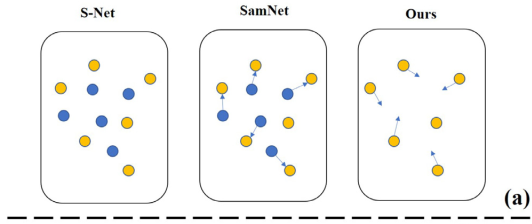
\includegraphics[width=\textwidth]{images/subfig-1.png}
%         \caption{}
        \label{fig:sub1}
    \end{subfigure}
    \begin{subfigure}[b]{0.5\textwidth}
        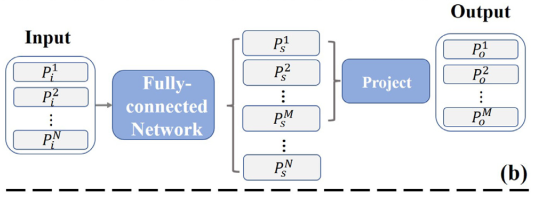
\includegraphics[width=\textwidth]{images/subfig-2.png}
%         \caption{}
        \label{fig:sub2}
    \end{subfigure}
    \begin{subfigure}[b]{0.5\textwidth}
        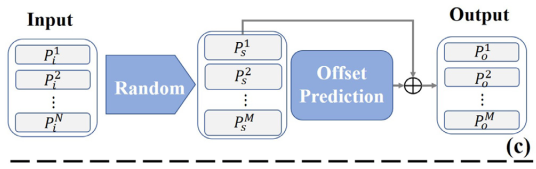
\includegraphics[width=\textwidth]{images/subfig-3.png}
%         \caption{}
        \label{fig:sub3}
    \end{subfigure}
    \captionsetup{justification=justified, labelsep=period}
    \caption{(a) shows the differences between learning-based sampling strategies, while (b) and (c) present the discrepancy between progress-net and our method in multi-resolution sampling.}
    \label{fig:fig1}
\end{figure}


Our contributions can be summarized as:
\begin{itemize}
 \item We propose a novel learning-based point cloud sampling framework named fast sampling network (FPN) by driving existing randomly sampled points to better positions;
 \item We introduce a hybrid training strategy to help FPN adapt to different sampling resolutions by randomly introducing selecting the resolution of initial points during training.
\end{itemize}


\section{Methodology}
\subsection{Basic Pipeline}
The basic pipeline of FPN is presented in \autoref{fig:fig2}. We aggregate global features from the input points with a set of multilevel perceptions (MLPs) and Max Pooling following PointNet \cite{qi2017pointnet}.

\subsection{Hybrid Training Strategy}
The achievement of HTS is presented as Algorithm \autoref{alg:algo-1}.

\subsection{Loss Function}
The range constraint can be presented as
\begin{equation}
 \mathcal{L}_{rc} = \frac{1}{N}\sum \|S_0 - S_i\|_2,
\end{equation}

For reconstruction-related tasks, it may be Chamfer Distance or Earth Mover Distance \cite{fan2017point} defined as
\begin{equation} \label{eqn:eqn1}
\begin{split}
\mathcal{L}_{task} & = \mathcal{L}_{CD}(S_1, S_2) \\
& = \frac{1}{2} \left (\frac{1}{|S_1|}\sum_{x \epsilon S_1}\min_{y \epsilon S_2} \|x-y\|_2 + \frac{1}{|S_2|}\sum_{x \epsilon S_2}\min_{y \epsilon S_1} \|x-y\|_2 \right ),
\end{split}
\end{equation}
or
\begin{equation}
 \mathcal{L}_{task} = \mathcal{L}_{EMD}(S_1, S_2) = \min_{\phi : S_1 \rightarrow S_2} \frac{1}{|S_1|}\sum_{x \epsilon S_1} \|x-\phi(x) \|_2.
\end{equation}
where $S_1$ and $S_2$ are input and output. $\phi$ is a bijection from $S_1$ to $S_2$.

\section{Experiments}
\subsection{Dataset and implementation details}
\label{subsec:dataset}
\begin{table}[H]
\captionsetup{justification=raggedright, labelfont=bf, labelsep=newline}
\caption{\RaggedRight The number of neurons in networks. $f_1$ , $f_2$ , $f_3$ are modules in \autoref{fig:fig2}.}
\label{table:table1}
\begin{tabularx}{0.5\textwidth}{>{\raggedright\arraybackslash}X >{\raggedright\arraybackslash}X >{\raggedright\arraybackslash}X >{\raggedright\arraybackslash}X}
\hline
& $f_1$ & $f_2$ & $f_3$ \\
\hline
MLPs & (128,256,256) & (128,256,256) & (128,128,3) \\
\hline
\end{tabularx}
\end{table}

\begin{table}[H]
\textbf{Table 2}
\captionsetup{labelformat=empty, justification=raggedright, labelsep=none}
\caption{\RaggedRight The comparison on optimal clustering.}
\label{table:table2}
\begin{tabularx}{0.5\textwidth}{>{\centering\arraybackslash}X >{\centering\arraybackslash}X >{\centering\arraybackslash}X >{\centering\arraybackslash}X >{\centering\arraybackslash}X }
\hline
Center & Iterations & 1 & 10 & 100 \\
\hline
16 & FPS & 2.43 & 2.00 & 1.98 \\
& Ours & \textbf{2.16} & \textbf{1.98} & \textbf{1.96} \\
32 & FPS & 1.20 & 1.02 & 1.00 \\
& Ours & \textbf{1.11} & \textbf{1.00} & \textbf{1.00} \\
\hline
\end{tabularx}
\end{table}
The hyper-parameter $\lambda$ is tuned on the validation split of ShapeNet. Detailed network structures are shown in \autoref{table:table1}.

\subsection{Discussion about clustering}
Except down-stream tasks such as reconstruction or recognition, down-sampled points can also be adopted as the initial clustering centers.
\begin{figure*}
\centering
 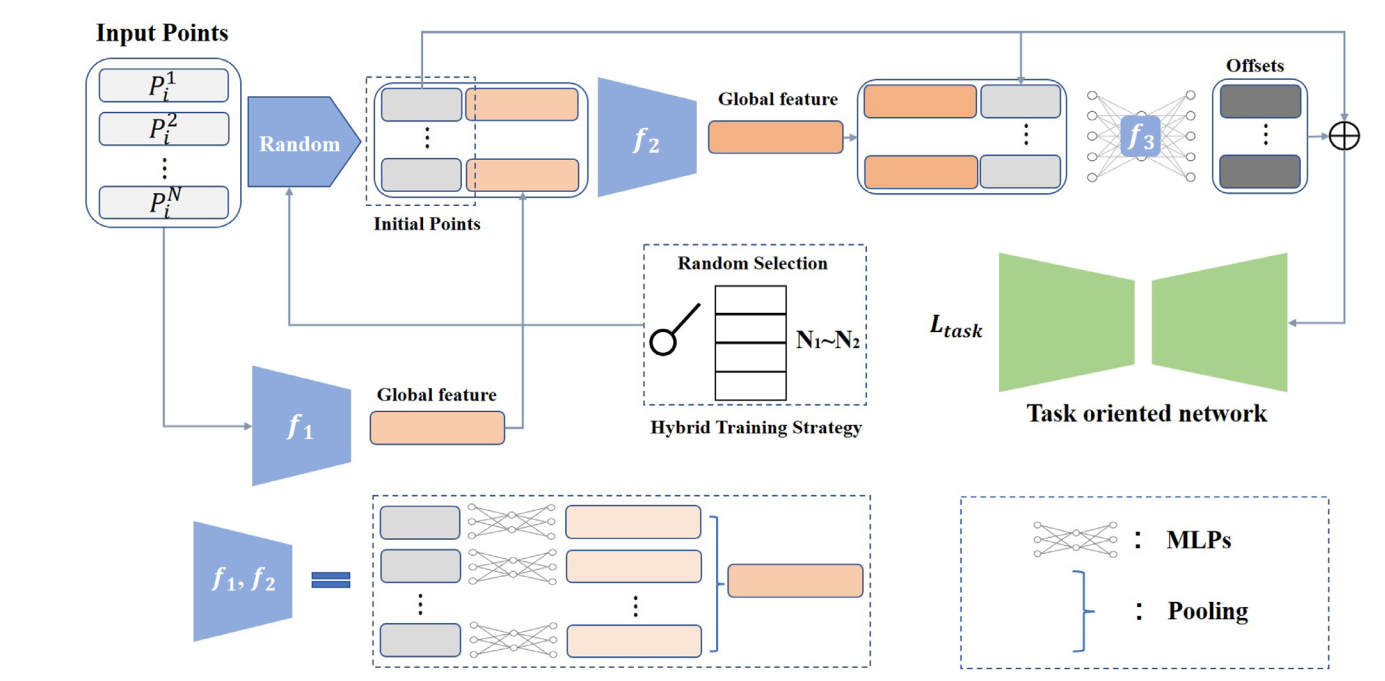
\includegraphics[width=\linewidth]{images/fig2.png}
 \captionsetup{justification=justified, labelsep=period}
 \caption{The whole pipeline of FPN. The + denotes element-wised addition. $f_1$ and $f_2$ aggregate features by MultiLayer Perceptrons(MLPs) and pooling, while $f_3$ is a group of MLPs to predict offsets from coordinates and features. The task network is corresponding to the specific task, such as point cloud recognition and reconstruction. $L_{task}$ is the loss constrained the task network.}
\label{fig:fig2}
\end{figure*}

The results are presented in \autoref{table:table2}.

\subsection{Ablation Study}
\textbf{The influence of range constraint.} Note that this is only conducted to observe the influence of range constraint weight $\lambda$ on sampling performances instead of the tuning of $\lambda$, which is chosen according to the val set introduced in \autoref{subsec:dataset}.

\begin{algorithm}[H]
\label{alg:algo-1}
\SetAlgoCaptionSeparator{}
\caption{Training with Hybrid Training Strategy}
\SetAlgoNoLine
\KwIn{data $X$, the number of iterations $iter$, the number of resolutions $m$;}
$prob_1, prob_2, \ldots, prob_m = \frac{1}{m}, \frac{1}{m}, \ldots, \frac{1}{m};$\\
\SetKwFor{For}{for}{do}{end for}
\For{$i=1$ \KwTo $iter$}
{
Select the resolution $r$ according to $prob_1,\ldots, prob_m$;\\Train FPN by descending gradient:$\Delta_{\theta_{FPN}}\mathcal{L}_{loss}\left(Y_{X, r}\right)$\\
}
\end{algorithm}

\section*{Data availability}
Data will be made available on request.

\section*{Acknowledgement}
We thank all reviewers and the editor for excellent contributions. This work is supported by the Key Research and Development Project of Zhejiang Province under Grant 2021C01035.

\printbibliography

\end{multicols}



\end{document}
